\documentclass[conference,a4paper]{IEEEtran}
\hbadness=99999

% Escritura mejorada de fórmulas matemáticas
\usepackage{amsmath}

% Inserción de gráficos
\usepackage{graphicx}

% Escritura de pseudocódigo
\usepackage[kw]{pseudo}

% Escritura mejorada de tablas
\usepackage{booktabs}

% Escritura mejorada de citas bibliográficas
\usepackage{cite}


% Macros traducidas
\def\contentsname{Índice general}
\def\listfigurename{Índice de figuras}
\def\listtablename{Índice de tablas}
\def\refname{Referencias}
\def\indexname{Índice alfabético}
\def\figurename{Fig.}
\def\tablename{TABLA}
\def\partname{Parte}
\def\appendixname{Apéndice}
\def\abstractname{Resumen}
% IEEE specific names
\def\IEEEkeywordsname{Palabras clave}
\def\IEEEproofname{Demostración}


\begin{document}

\title{Filtrado de correo electrónico no deseado}

\author{
\IEEEauthorblockN{Juan Antonio Ortiz Guerra}
  \IEEEauthorblockA{
    \textit{Dpto. Ciencias de la Computación e Inteligencia Artificial}\\
    \textit{Universidad de Sevilla}\\
    Sevilla, España\\
    Correo electrónico UVUS: juaortgue@alum.us.es\\
    Correo electrónico de contacto:juanantonioortizguerra@gmail.com}
    
  \and 
 
  \IEEEauthorblockN{Jesús Páez Páez}
  \IEEEauthorblockA{
    \textit{Dpto. Ciencias de la Computación e Inteligencia Artificial}\\
    \textit{Universidad de Sevilla}\\
    Sevilla, España\\
    Correo electrónico UVUS: jespaepae@alum.us.es \\
    Correo electrónico de contacto:jesuspaezpaez@gmail.com}
  
  
}
\maketitle

% Resumen
\begin{abstract}
El objetivo principal de este trabajo es la construcción de un filtro de 		correo electrónico no deseado mediante el uso de técnicas de procesamiento del lenguaje natural.

Con la realización de este proyecto hemos consolidado conocimientos sobre métodos de procesamiento de lenguaje natural para clasificar documentos, así como procedimientos para evaluar el rendimiento de los distintos filtros construidos.
\end{abstract}

% Palabras claves
\begin{IEEEkeywords}
  Filtro, spam, correo electrónico, bolsa de palabras, clasificador, matriz de confusión.
\end{IEEEkeywords}


\section{Introducción}
En la actualidad es cada vez más común recibir correos electrónicos no deseados. Estos correo no son solo una incomodidad, sino que también pueden suponer un peligro para nuestra seguridad y privacidad. Es por ello que la creación de filtros capaces de identificar correos electrónicos no deseados es una necesidad. Por este motivo, en este trabajo construiremos dos filtros capaces de identificar si un correo es legítimo o no es deseado. \\

Para la realización de dichos filtros hemos usado  técnicas de procesamiento de lenguaje natural, basándonos en la teoría que se nos proporciona en la asignatura~\cite{b1}, además de algún trabajo relacionado que se mencionará en secciones posteriores. \\

Por otra parte, para la selección del mejor filtro hemos escogido algunas métricas que aparecen en el apartado de evaluación y selección de modelos de la teoría que se ha impartido en la asignatura sobre aprendizaje automático~\cite{b2}. \\

Este documento se divide en cinco secciones principales:
\begin{enumerate}
\item \textit{Introducción}: Indicamos el contexto en el que se desarrolla el trabajo presentado.
\item \textit{Preliminares}: Hacemos una introducción de las técnicas empleadas y se mencionan trabajos relacionados con este proyecto.
\item \textit{Metodología}: Describimos el método implementado en el trabajo.
\item \textit{Resultados}: Detallamos tanto los experimentos realizados como los resultados obtenidos.
\item \textit{Conclusiones}: Resumimos el trabajo realizado y exponemos ideas de mejora y trabajo futuro.
\end{enumerate}


\section{Preliminares}

A continuación realizamos una breve introducción de las técnicas empleadas y mencionamos trabajos relacionados con el proyecto.

\subsection{Métodos empleados}

\subsubsection{Lectura de correos}
Para la lectura de correos usamos la librerías email~\cite{b3} y glob~\cite{b4}. En nuestro proyecto hemos realizado dos lecturas diferentes, una en la que nos quedamos con los asuntos de los correos y otra en la que añadimos además los cuerpos (analizaremos ambas lecturas en secciones posteriores). Además, usamos técnicas de preprocesamiento de datos para eliminar aquella información irrelevante de los asuntos, como los signos de puntuación o las "palabras vacías". Para ello usamos la librería nltk~\cite{b5}.\\

\subsubsection{Creación de filtros}
Para la creación de filtros, en primer lugar seleccionamos un vocabulario de términos a partir del conjunto de correos que hemos analizado. \\

Después de esto, construimos dos filtros, uno de ellos usando el modelo de lenguaje de bolsa de palabras, que representa cada documento como un vector en el que cada elemento indica el número de veces que aparece un término en ese documento~\cite{b1}, además de usar Naive Bayes multinomial como modelo clasificador. \\

Por otra parte, para el segundo filtro usamos como modelo de lenguaje tf-idf, que disminuye la relevancia de los términos que son muy comunes en varios documentos, mientras que la aumenta en el caso de aquellas palabras que son muy comunes en pocos documentos~\cite{b1}, y como modelo clasificador usamos el modelo clasificador kNN. \\

\subsubsection{Evaluación del rendimiento de filtros}
Para evaluar el rendimiento de los filtros creados, en primer lugar dividimos el directorio que contiene todos los correos en dos directorios, uno con un conjunto de entrenamiento y otro con un conjunto de validación. Para ello utilizamos la biblioteca que se nos recomendó, split-folders~\cite{b5}, haciendo que el conjunto de entrenamiento contenga el 80\% de los correos iniciales, mientras que el conjunto de validación abarca el 20\%. \\

Después de esto, entrenamos los filtros usando el conjunto de entrenamiento y evaluamos su rendimiento a través del uso de matrices de confusión sobre el conjunto de validación. Para ello hacemos uso de la librería sklearn~\cite{b7} para el cálculo de las matrices de confusión, y las librerías seaborn~\cite{b8} y matpotlib~\cite{b9} para su visualización. \\

Finalmente, para la elección del mejor filtro comparamos algunas métricas que podemos calcular a partir de las matrices de confusión, tales como:
\begin{itemize}
\item Tasa de acierto: Proporción de ejemplos clasificados correctamente~\cite{b2}: \[ acc = \frac{1}{|D|} \sum_{i=1}^{m} c_{ii} \]
donde $c_{ii}$ representa los elementos de la diagonal de la matriz de confusión y $|D|$ el número total de ejemplos en el conjunto de validación.
\item Tasa de error: Proporción de ejemplos clasificados incorrectamente~\cite{b2}. \[ err = \frac{1}{|D|} \sum_{i,j=1, i\neq j}^{m} c_{ij} \]
donde $c_{ij}$ representa los elementos que no pertenecen a la diagonal de la matriz de confusión y $|D|$ el número total de ejemplos en el conjunto de validación.
\item Tasa de verdaderos positivos: Proporción de ejemplos positivos clasificados correctamente~\cite{b2}: $$tpr = \frac{VP}{VP+FN}$$.
\item Tasa de verdaderos negativos: Proporción de ejemplos negativos clasificados correctamente~\cite{b2}: $$tnr = \frac{FN}{VP+FN}$$.
\item Tasa de falsos positivos: Proporción de ejemplos positivos clasificados incorrectamente~\cite{b2}: $$fpr = \frac{VP}{VP+FN}$$.
\item Tasa de falsos negativos: Proporción de ejemplos negativos clasificados incorrectamente~\cite{b2}: $$fnr = \frac{VP}{VP+FN}$$.
\end{itemize}

\subsection{Trabajo Relacionado}

Como trabajo relacionado cabe destacar un blog~\cite{b10} en el que se realiza una clasificación de correos electrónicos no deseados, y del que nos hemos basado, sobre todo, para la representación de las matrices de confusión para la evaluación del rendimiento de los filtros construidos.

\section{Metodología}
En esta sección describiremos la metodología usada para la creación de los dos filtros. \\

En primer lugar, para la selección del vocabulario que usaremos para el entrenamiento de los dos filtros hemos leído y analizado los correos de dos formas distintas: \\
\begin{itemize}
\item Leemos únicamente los asuntos de los correos. Haciendo esto, el entrenamiento del filtro requiere muy poco tiempo y, además, puede leer todos los correos perteneciente al conjunto de entrenamiento. Sin embargo, al leer sólo los asuntos puede que no incluyamos información relevante en el vocabulario que aparezca en otras partes del correo como puede ser el cuerpo. \\

Esto lo hacemos con una función llamada \texttt{readEmails}, que al recibir una url con la ruta del directorio que contiene los correos electrónicos devuelve una lista en el que cada elemento es el asunto del correo correspondiente. \\

\item Leemos y analizamos además los cuerpos de los correos, añadiendo así más información al vocabulario de términos y creando filtros más precisos. Sin embargo, con el método que hemos implementado es imposible que se realice la lectura de todos los correos electrónicos del conjunto de entrenamiento ya que consume demasiado tiempo, por lo que solo entrenamos los filtros con un total de 100 correos. \\

Esto lo hacemos con una función llamada \texttt{readEmailsWithBody}, que al recibir una url con la ruta del directorio que contiene los correos devuelve una lista en la que cada elemento es la concatenación del asunto con el cuerpo del correo. \\
\end{itemize}

Después de la lectura de los correos, utilizamos un método llamado \texttt{cleanText} para eliminar tanto los signos de puntuación como las "palabras vacías", que son aquellas palabras que no aportan información relevante. Este método recibe como entrada un texto y devuelve el mismo texto sin signos de puntuación y eliminando las "palabras vacías". \\

Una vez que hemos leído los correos y hemos eliminado la información relevante, ya tenemos el vocabulario con el que se van a crear los filtros que estamos buscando. \\

\subsection{Filtro Naive Bayes Multinomial}
Para crear el primer filtro, usaremos como modelo de lenguaje la bolsa de palabras~\cite{b11} y como modelo clasificador Naive Bayes multinomial~\cite{b12}. \\

En primer lugar, transformamos la lista con los textos de los correos en una matriz, en la que cada fila representa un correo electrónico, y cada columna un término, de manera que cada elemento de la matriz indica el número de veces que se repite el término de la columna en el documento de la fila. Esto se realiza con la librería que implementa el modelo de bolsa de palabras~\cite{b11}. \\

A continuación, inicializamos el modelo clasificador, que tiene un parámetro \texttt{alpha} indicando el hiperparámetro de suavizado de Laplace para evitar que alguna estimación del modelo sea cero. Más adelante evaluaremos el rendimiento del filtro con distintos valores del hiperparámetro de suavizado. \\

Después de esto, creamos un array en el que cada elemento representa un correo electrónico del conjunto de entrenamiento, y el valor de ese elemento del array será uno si el correo es un correo electrónico no deseado o cero si es legítimo. \\

Con este array y la matriz conseguida anteriormente, entrenamos el modelo clasificador usando la librería correspondiente~\cite{b12}. Una vez hecho esto, ya podemos clasificar correos usando dicha librería. Para ello, leemos los correos del conjunto de validación de la misma forma que lo hicimos con el conjunto de entrenamiento. \\

Finalmente le pedimos al filtro que clasifique los correos del conjunto de validación y evaluamos los resultados de este. Este último paso lo analizaremos en la sección de Resultados. \\

\subsection{Filtro KNN}
Para crear este filtro, usaremos como modelo de lenguaje tf-idf~\cite{b13} y como modelo clasificador knn~\cite{b14}. \\

Al igual que con el filtro en el que usamos naive bayes multinomial, tenemos que transformar la lista con los textos de los correos analizados en una matriz para usar correctamente la librería que implementa tf-idf~\cite{b13}. En este caso, al igual que con el filtro anterior, las filas se corresponden con los distintos correos, mientras que las columnas identifican a los diferentes términos del vocabulario. Sin embargo, en este modelo el valor de cada elemento de la matriz representa el valor tf-idf de un término en un documento. \\

Después de esto inicializamos el modelo clasificador~\cite{b14}, que tiene un parámetro $n\_neighbors$ que indica el número de los vecinos más cercanos que se necesitan para clasificar los documentos. \\

Al igual que en el filtro anterior, creamos un array en el que cada elemento representa un correo electrónico del conjunto de entrenamiento, y el valor de ese elemento del array será uno si el correo es un correo electrónico no deseado o cero si es legítimo. \\

Con el array y la matriz conseguida anteriormente, entrenamos el modelo clasificador knn usando métodos de la librería que implementa dicho clasificador~\cite{b14}. Al hacer esto, el modelo está entrenado y preparado para poder clasificar documentos.\\

Para finalizar le pedimos al filtro que clasifique los correos pertenecientes al conjunto de validación, para así poder hacer una matriz de confusión y poder evaluar el rendimiento del filtro. Los resultados del análisis se mostrarán en la siguiente sección. \\

\section{Resultados}

En esta sección se detallarán tanto los experimentos realizados como los
resultados conseguidos. Como ya comentamos en secciones anteriores, para evaluar el rendimiento de los filtros construidos realizaremos varios experimentos construyendo matrices de confusión y analizando algunas métricas obtenidas a partir de estas. \\

Analizamos en primer lugar cada filtro por separado, teniendo en cuenta también si la lectura la hemos realizado añadiendo únicamente los asuntos de los correos o, además, también los cuerpos. \\

\subsection{Filtro Naive Bayes Multinomial}
En primer lugar para $alpha=1$: \\

\begin{figure}[h]
  \centering
  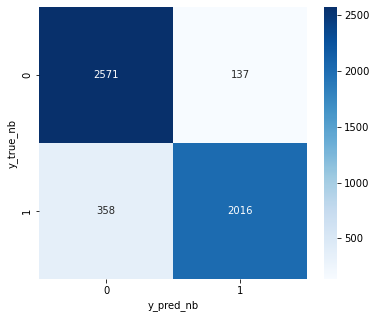
\includegraphics[width=75mm]{nb_1}
  \caption{Matriz de confusión para $alpha=1$}
  \label{fig:ejemplo}
\end{figure}

A partir de esta matriz de confusión podemos sacar las siguientes métricas:

\begin{center}
\begin{tabular}[h]{ |c|c|c|c|c|c|c| } 
 \hline
 Métrica & acc & err & tpr & tnr & fpr & fnr \\ 
 \hline
 Valor & 0.903 & 0.097 & 0.949 & 0.849 & 0.051 & 0.151 \\ 
 \hline
\end{tabular}
\end{center}

Realizamos el mismo procedimiento para distintos valores de $alpha$ y comprobamos qué es más óptimo:\\

\begin{figure}[h]
  \centering
  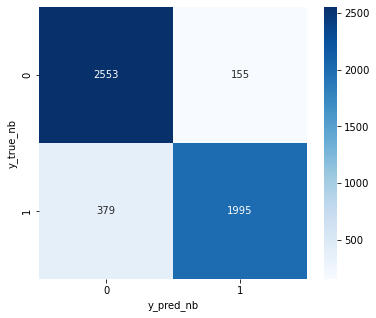
\includegraphics[width=75mm]{nb_5}
  \caption{Matriz de confusión para $alpha=5$}
  \label{fig:ejemplo}
\end{figure}

A partir de esta matriz de confusión podemos sacar las siguientes métricas:

\begin{center}
\begin{tabular}[H]{ |c|c|c|c|c|c|c| }
 \hline
 Métrica & acc & err & tpr & tnr & fpr & fnr \\ 
 \hline
 Valor & 0.895 & 0.105 & 0.943 & 0.84 & 0.057 & 0.16 \\ 
 \hline
\end{tabular}
\end{center}

\begin{figure}[h]
  \centering
  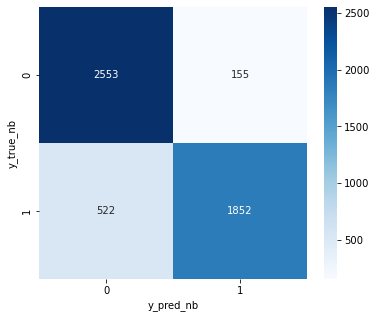
\includegraphics[width=75mm]{nb_30}
  \caption{Matriz de confusión para $alpha=30$}
  \label{fig:ejemplo}
\end{figure}

A partir de esta matriz de confusión podemos sacar las siguientes métricas:

\begin{center}
\begin{tabular}[h]{ |c|c|c|c|c|c|c| } 
 \hline
 Métrica & acc & err & tpr & tnr & fpr & fnr \\ 
 \hline
 Valor & 0.867 & 0.133 & 0.943 & 0.78 & 0.057 & 0.22 \\ 
 \hline
\end{tabular}
\end{center}

Como podemos comprobar, a medida que aumentamos el valor del hiperparámetro de suavizado el filtro empeora. A pesar de que el número de correos legítimos que clasifica correctamente no cambia mucho, el número de correos spam que clasifica incorrectamente sí que aumenta de una forma más notable. Por lo tanto en este caso la mejor opción es mantener el valor del hiperparámetro de suavizado bajo, es decir, 1. \\

Vamos a analizar cuál es el rendimiento del mismo filtro, pero esta vez usando la lectura en la que añadimos también los cuerpos de los correos en el vocabulario del modelo. Usamos los mismos valores del hiperparámetro de suavizado de Laplace: \\

\begin{figure}[h]
  \centering
  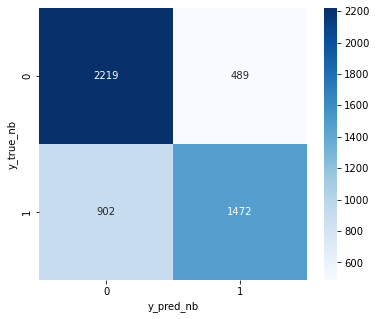
\includegraphics[width=75mm]{nb_body_1}
  \caption{Matriz de confusión para $alpha=1$}
  \label{fig:ejemplo}
\end{figure}

A partir de esta matriz de confusión podemos sacar las siguientes métricas:

\begin{center}
\begin{tabular}[h]{ |c|c|c|c|c|c|c| } 
 \hline
 Métrica & acc & err & tpr & tnr & fpr & fnr \\ 
 \hline
 Valor & 0.726 & 0.274 & 0.62 & 0.849 & 0.181 & 0.38 \\ 
 \hline
\end{tabular}
\end{center}

\begin{figure}[h]
  \centering
  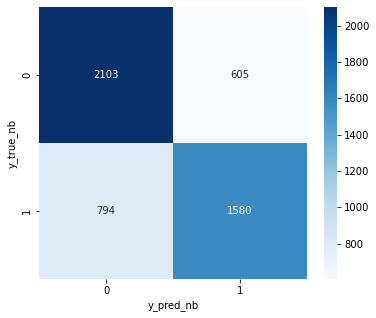
\includegraphics[width=75mm]{nb_body_30}
  \caption{Matriz de confusión para $alpha=30$}
  \label{fig:ejemplo}
\end{figure}

A partir de esta matriz de confusión podemos sacar las siguientes métricas:

\begin{center}
\begin{tabular}[h]{ |c|c|c|c|c|c|c| } 
 \hline
 Métrica & acc & err & tpr & tnr & fpr & fnr \\ 
 \hline
 Valor & 0.725 & 0.275 & 0.777 & 0.666 & 0.222 & 0.333 \\ 
 \hline
\end{tabular}
\end{center}

Como podemos ver, al analizar las métricas observamos que la tasa de acierto se mantiene similar para ambos valores del hiperparámetro de suavizado. Sin embargo, el modelo tiende a clasificar mejor los correos que son spam para valores de hiperparámetros mayores, mientras que empeora al clasificar correos que son legítimos. \\

Hay que tener en cuenta que este filtro está entrenado con muchos menos correos que el que analiza únicamente los asuntos, por lo que es normal que los valores de las métricas sean peores.


\subsection{Filtro KNN}
En primer lugar para $n\_neighbors=5$: \\

\begin{figure}[h]
  \centering
  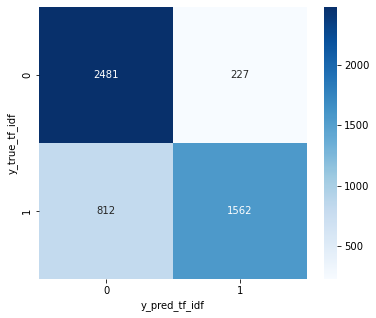
\includegraphics[width=65mm]{knn_5}
  \caption{Matriz de confusión para $n\_neighbors=5$}
  \label{fig:ejemplo}
\end{figure}

A partir de esta matriz de confusión podemos sacar las siguientes métricas:

\begin{center}
\begin{tabular}[bp!]{ |c|c|c|c|c|c|c| } 
 \hline
 Métrica & acc & err & tpr & tnr & fpr & fnr \\ 
 \hline
 Valor & 0.796 & 0.204 & 0.916 & 0.658 & 0.084 & 0.342 \\ 
 \hline
\end{tabular}
\end{center}

Realizamos el mismo procedimiento para distintos valores de $n\_neighbors$ y comprobamos qué es más óptimo: \\

\begin{figure}[h]
  \centering
  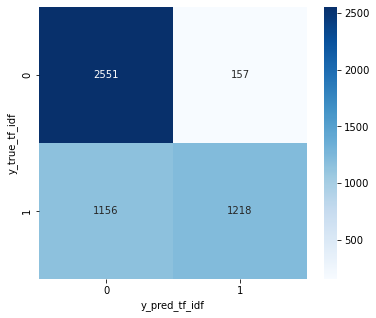
\includegraphics[width=65mm]{knn_15}
  \caption{Matriz de confusión para $n\_neighbors=15$}
  \label{fig:ejemplo}
\end{figure}

A partir de esta matriz de confusión podemos sacar las siguientes métricas:

\begin{center}
\begin{tabular}{ |c|c|c|c|c|c|c| }
 \hline
 Métrica & acc & err & tpr & tnr & fpr & fnr \\ 
 \hline
 Valor & 0.742 & 0.258 & 0.942 & 0.526 & 0.058 & 0.474 \\ 
 \hline
\end{tabular}
\end{center}

\begin{figure}[h]
  \centering
  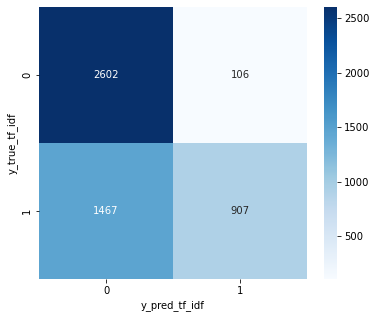
\includegraphics[width=75mm]{knn_31}
  \caption{Matriz de confusión para $n\_neighbors=31$}
  \label{fig:ejemplo}
\end{figure}

A partir de esta matriz de confusión podemos sacar las siguientes métricas:

\begin{center}
\begin{tabular}[h]{ |c|c|c|c|c|c|c| } 
 \hline
 Métrica & acc & err & tpr & tnr & fpr & fnr \\ 
 \hline
 Valor & 0.69 & 0.31 & 0.961 & 0.382 & 0.039 & 0.618 \\ 
 \hline
\end{tabular}
\end{center}

En este caso, a medida que va aumentando el hiperparámetro k, peor es el rendimiento del filtro ya que aunque mejore en la clasificación de los correos electrónicos legítimos, empeora excesivamente en la clasificación de los correos electrónicos no deseados, por lo que en este caso el rendimiento del filtro es mejor cuanto menor sea el valor del hiperparámetro k. \\

Finalmente analizamos cuál es el comportamiento de dicho filtro pero añadiendo los cuerpos en la lectura de los correos: \\

\begin{figure}[h]
  \centering
  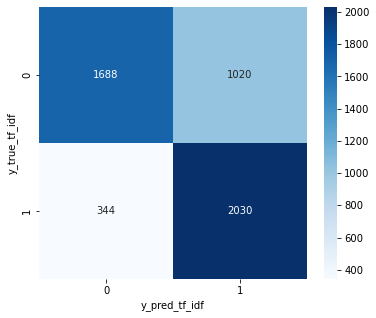
\includegraphics[width=75mm]{knn_body_15}
  \caption{Matriz de confusión para $n\_neighbors=15$}
  \label{fig:ejemplo}
\end{figure}

A partir de esta matriz de confusión podemos sacar las siguientes métricas:

\begin{center}
\begin{tabular}{ |c|c|c|c|c|c|c| }
 \hline
 Métrica & acc & err & tpr & tnr & fpr & fnr \\ 
 \hline
 Valor & 0.728 & 0.272 & 0.623 & 0.855 & 0.377 & 0.145 \\ 
 \hline
\end{tabular}
\end{center}

\begin{figure}[h]
  \centering
  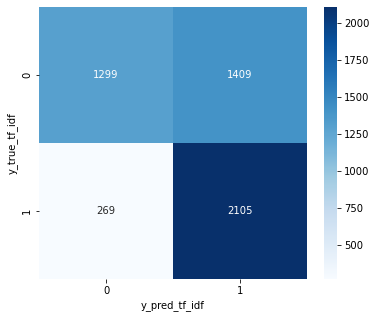
\includegraphics[width=90mm]{knn_body_31}
  \caption{Matriz de confusión para $n\_neighbors=31$}
  \label{fig:ejemplo}
\end{figure}

A partir de esta matriz de confusión podemos sacar las siguientes métricas:

\begin{center}
\begin{tabular}[h]{ |c|c|c|c|c|c|c| } 
 \hline
 Métrica & acc & err & tpr & tnr & fpr & fnr \\ 
 \hline
 Valor & 0.67 & 0.33 & 0.48 & 0.887 & 0.52 & 0.113 \\ 
 \hline
\end{tabular}
\end{center}

Al contrario que en el caso anterior en el que únicamente se leían los asuntos de los correos, en este filtro al aumentar el hiperparámetro k mejora en la clasificación de correos electrónicos no deseados, pero empeora en la clasificación de correos legítimos. \\

En general el filtro funciona mejor cuando solo lee los asuntos de los correos en lugar de cuando también añade los cuerpos. Sin embargo, en el segundo caso sólo se han tenido como conjunto de entrenamiento un total de 100 correos por lo que es muy probable que si se entrenara con el mismo conjunto de entrenamiento, el filtro funcionaría mejor al analizar también los cuerpos de los correos. \\

Por tanto, el filtro que hemos escogido finalmente ya que consideramos que es más óptimo después de la evaluación del rendimiento de los diferentes filtros ha sido el que usa como modelo de lenguaje bolsa de palabras y como modelo de clasificación naive bayes multinomial con un hiperparámetro de suavizado de Laplace de 1. \\

\section{Conclusiones}

Con la realización de este proyecto hemos afianzado conceptos sobre el procesamiento del lenguaje natural y sobre el aprendizaje automático, construyendo varios tipos de filtros de clasificación de correos electrónicos y analizando dichos filtros usando técnicas aprendidas en la asignatura para elegir el más adecuado. \\

Como hemos podido comprobar, el rendimiento del filtro que usa como modelo del lenguaje tf-idf y como modelo clasificador knn no ha sido igual que el otro filtro. \\

Al analizar las métricas obtenidas a partir de las distintas matrices de confusión calculadas, concluimos que el mejor filtro es aquel que tenga la tasa de acierto más alta, o lo que es lo mismo, el filtro que tenga la tasa de error más baja. \\

Por tanto el resultado final es un filtro de correo electrónico que usa naive bayes multinomial como modelo clasificador con un hiperparámetro de suavizado de Laplace de 1, y bolsa de palabras como modelo de lenguaje. \\

Sin embargo, es un filtro que se podría mejorar bastante, ya que se podría optimizar la lectura de los correos electrónicos y las técnicas para procesar dichos correos, ya sea bien filtrando los cuerpos de forma que no consuman tanto tiempo de ejecución o teniendo en cuenta algunos atributos de los mensajes además del asunto. \\

\begin{thebibliography}{00}
\bibitem{b1} Procesamiento del lenguaje natural. Dpto. Ciencias de la Computación e Inteligencia Artificial. Universidad de Sevilla.
\bibitem{b2} Aprendizaje Automático. Dpto. Ciencias de la Computación e Inteligencia Artificial. Universidad de Sevilla.
\bibitem{b3} Librería email de python. https://docs.python.org/3/library/email.html\#module-email.
\bibitem{b4} Librería glob de python. https://docs.python.org/3/library/glob.html\#module-glob.
\bibitem{b5} Librería nltk de python. https://www.nltk.org/
\bibitem{b6} Librería split-folders de python. https://pypi.org/project/split-folders/ 
\bibitem{b7} Librería sklearn.metrics.confusion\_matrix de python. https://scikit-learn.org/stable/modules/generated/sklearn.metrics.confusion\_matrix.html
\bibitem{b8} Librería seaborn de python. https://seaborn.pydata.org/
\bibitem{b9} Librería matpotlib de python. https://matplotlib.org/
\bibitem{b10} Trabajo relacionado sobre clasificación de correos electrónicos. https://www.milindsoorya.com/blog/build-a-spam-classifier-in-python
\bibitem{b11} Librería para implementar el modelo de bolsa de palabras. https://scikit-learn.org/stable/modules/generated/sklearn.feature\_extraction.text.CountVectorizer.html
\bibitem{b12} Librería de python para implementar naive bayes multinomial https://scikit-learn.org/stable/modules/generated/sklearn.naive\_bayes.MultinomialNB.html
\bibitem{b13} Librería de python para implementar tf-idf. https://scikit-learn.org/stable/modules/generated/sklearn.feature\_extraction.text.TfidfVectorizer.html
\bibitem{b14} Librería de python para implementar knn. https://scikit-learn.org/stable/modules/generated/sklearn.neighbors.KNeighborsClassifier.html
\end{thebibliography}

\end{document}
